
\documentclass[a4paper,12pt]{article}
\usepackage{graphicx}
\usepackage[table,xcdraw]{xcolor}
\usepackage{geometry}
\usepackage{float}
\usepackage[colorlinks=false, hidelinks]{hyperref}
\usepackage{fancyhdr}% For page numbering
\geometry{top=1in,bottom=1in,left=1in,right=1in}
\usepackage{listings}
\usepackage{xcolor}
\usepackage{hyperref}
\pagestyle{empty}


\begin{document}

\begin{center}
    \vspace{0.2cm}
    \textbf{\large{Course Title: Software Engineering \& ISD Lab}}\\
    \vspace{0.2cm}
    \textbf{Course Code: CSE-404}\\
    \vspace{0.2cm}
    \textbf{4\textsuperscript{th}Year 1\textsuperscript{st}Semester Examination 2023}\\
    \vspace{0.5cm}
    \textbf{Date of Submission: \today}\\

    \vspace{1.5cm}
    
\includegraphics[width=0.35\textwidth]{images/logo.png}\\ % Replace 'logo.png' with the correct path if you have the university logo image
    \vspace{1cm}

    \textbf{Submitted to}\\
    \vspace{0.2cm}
    \textbf{\href{https://juniv.edu/teachers/musfique.anwar}{Dr. Md Musfique Anwar}}\\
    {Professor}\\
    \vspace{0.2cm}
    \textbf{\href{https://juniv.edu/teachers/hkabir}{Dr. Md. Humayun Kabir}}\\
    {Professor}\\


    \vspace{1cm}

    \begin{table}[h!]
        \centering
        \arrayrulecolor{black}
        \begin{tabular}{|c|c|c|c|}
            \hline
            \rowcolor[HTML]{2F4F4F} % Changed header background color to dark slate gray
            {\color[HTML]{FFFFFF}\textbf{Sl}}& {\color[HTML]{FFFFFF}\textbf{Class Roll}}& {\color[HTML]{FFFFFF}\textbf{Exam Roll}}& {\color[HTML]{FFFFFF}\textbf{Name}}\\ \hline
            \rowcolor[HTML]{B0E0E6}
            \textbf{1}& \textbf{408} & \textbf{202220} & \textbf{Sudipta Singha} \\ \hline
       
        \end{tabular}
    \end{table}

    \vspace{1cm}

    Department of Computer Science and Engineering\\
    Jahangirnagar University\\
    Savar, Dhaka, Bangladesh\\
\end{center}

\newpage

\tableofcontents

\newpage
\pagestyle{fancy}
\fancyhf{}
\fancyfoot[C]{\thepage} % Page number in the center of the footer
\section{Introduction}
Test-Driven Development (TDD) is an agile software development methodology where tests are written before the
code. It emphasizes creating comprehensive test suites and automating tests to ensure efficiency and
reliability in software development. This report details my individual contribution and reflections on the
adoption and practice of TDD during our project’s development phase, starting from Sprint 2.
\section{Individual Contribution to TDD Practice}
\begin{enumerate}
    \item \textbf{Tool Selection:}
        \begin{itemize}
            \item After discussing with the team, we decided to use those tools to support TDD effectively:
                \begin{itemize}
                    \item Django's Built-in Test Framework  
                    \item Hardcoded mock data
                    \item Github actions for automating test execuation and integration
                \end{itemize}
            \item Justification: These tools are lightweight, versatile, and well-integrated into our
                development stack.
        \end{itemize}
    \item \textbf{Test Design}
        \begin{itemize}
            \item I designed initial test cases for core modules:
                \begin{itemize}
                    \item \textbf{Create Account: }Write test case for account creation feature.
                    \item \textbf{Dispense Medicine to Patients: }Write test case for dispense medicine to
                        patients
                    \item \textbf{Update Stock information: }Write test case for update stock information for
                        medicines.
                \end{itemize}
            \item Collaborated with the team to review and refine these test cases.
        \end{itemize}
    \item \textbf{Implementation}
        \begin{itemize}
            \item Writing Tests: Developed unit tests for the user authentication module, focusing on boundary
                cases and invalid inputs.
            \item Refactoring: Adjusted existing code to ensure it was testable and adhered to TDD principles.
            \item Automation: Configured github actions to automatically run tests upon code push, ensuring CI
                alignment.
        \end{itemize}
\end{enumerate}
\begin{figure}[H]
    \centering
    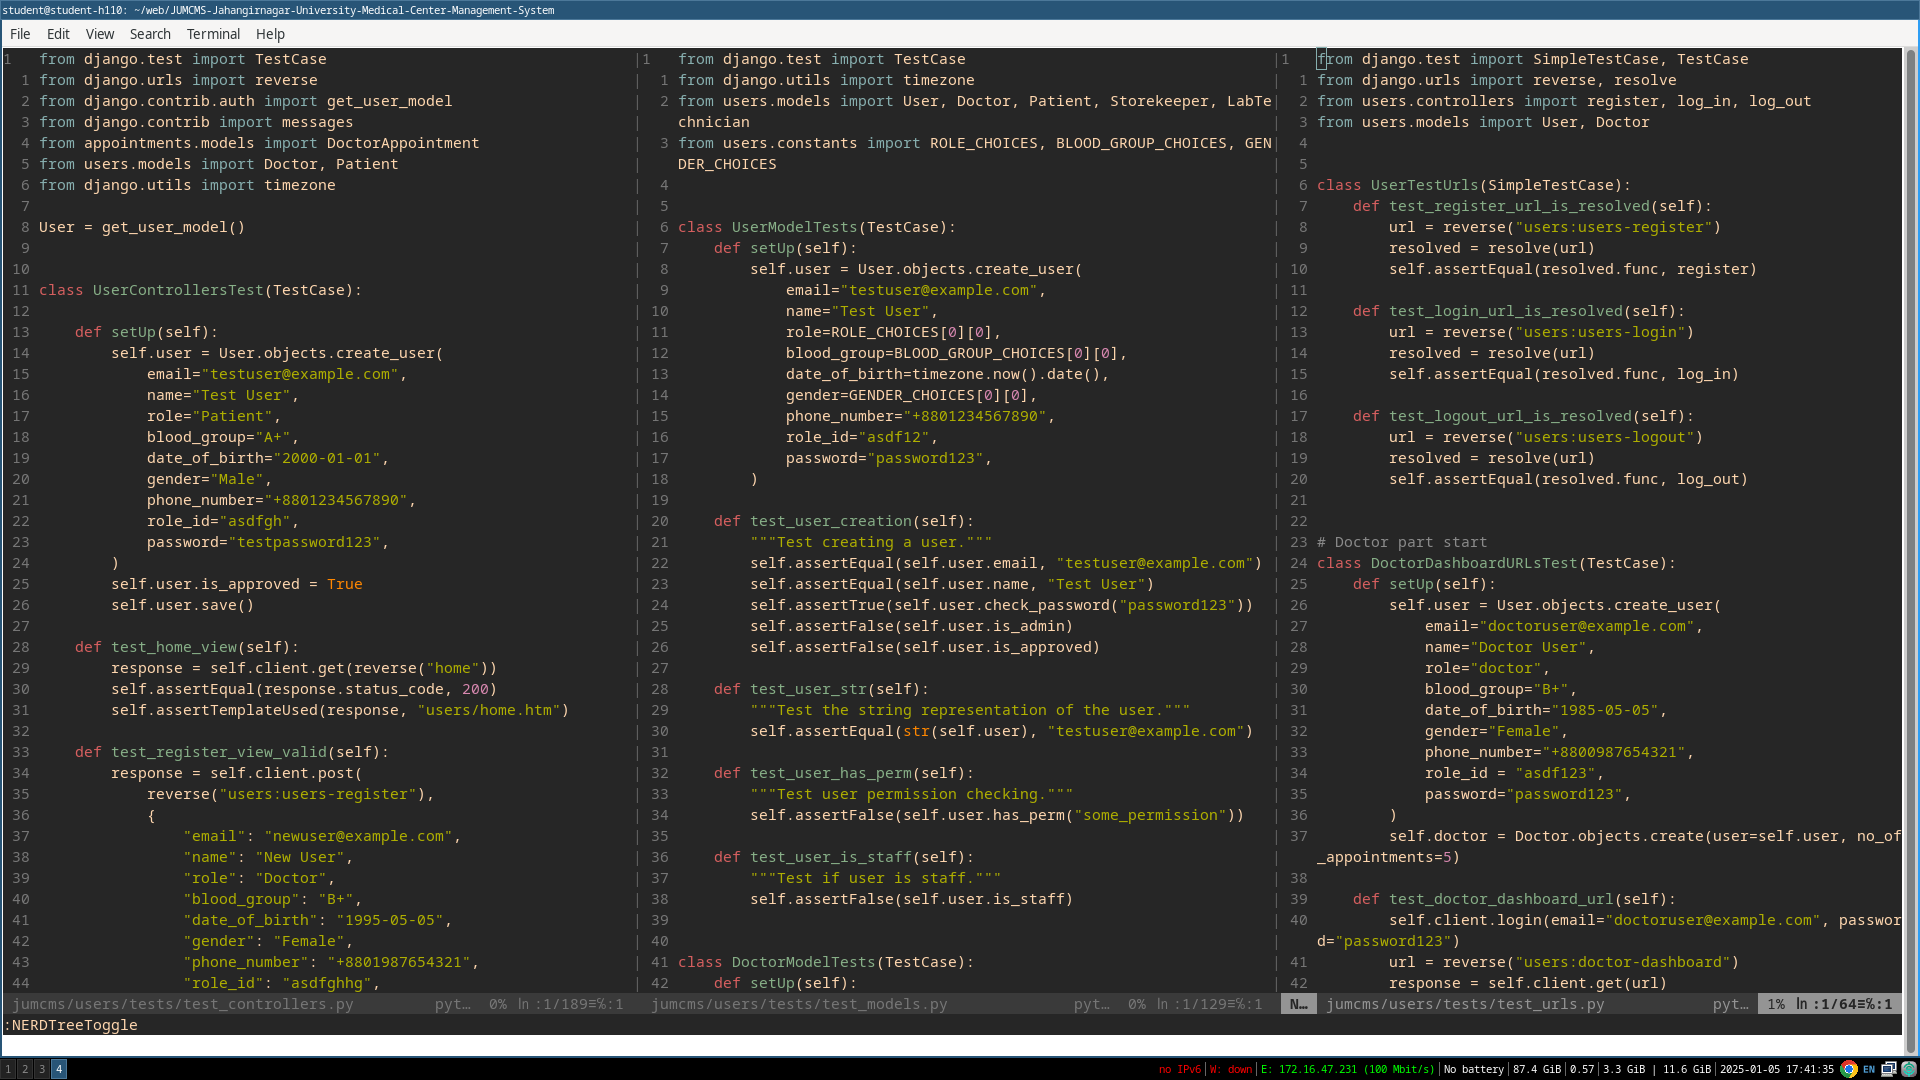
\includegraphics[width=1\textwidth]{images/TDD1.png}
    \caption{Testing code for create account feature}
    \label{fig:tdd1}
\end{figure}
\begin{figure}[H]
    \centering
    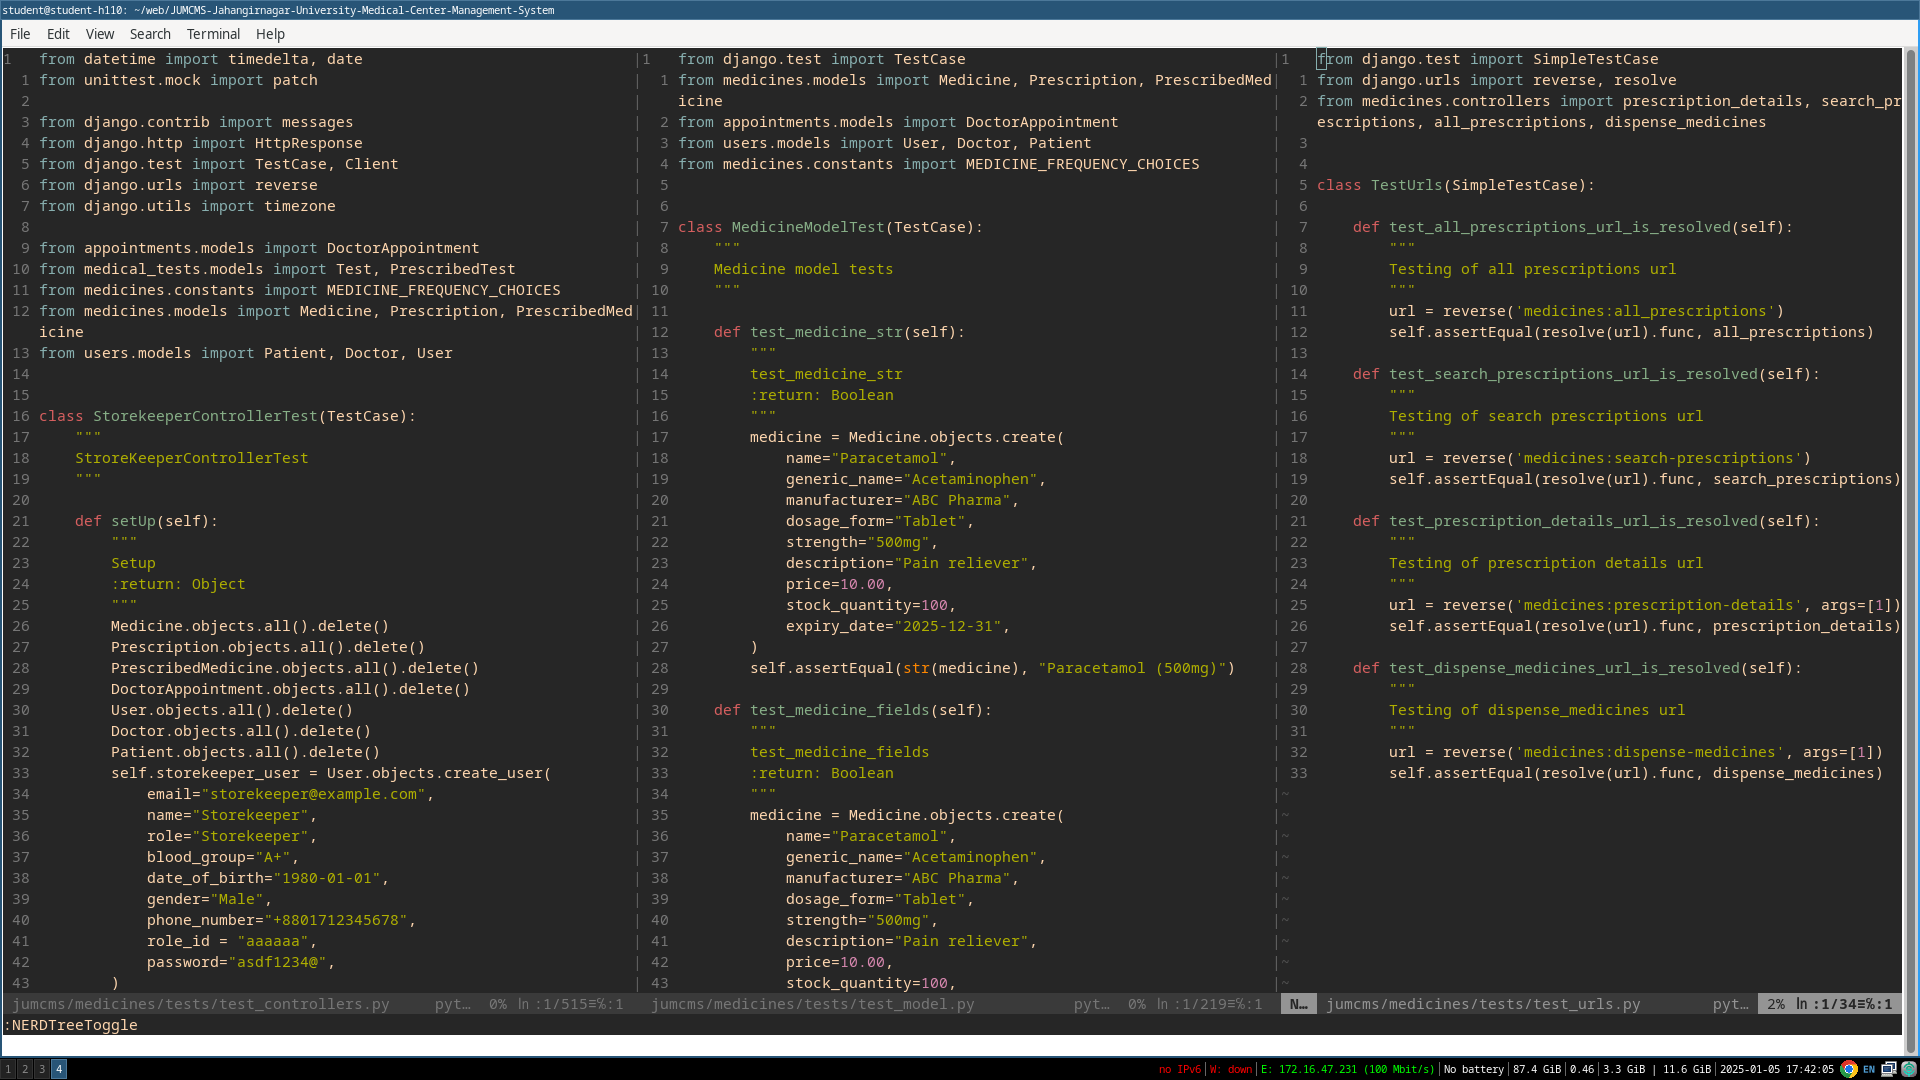
\includegraphics[width=1\textwidth]{images/TDD2.png}
    \caption{Testing code for dispense medicine to patients and update stock information feature}
    \label{fig:tdd2}
\end{figure}
\begin{figure}[H]
    \centering
    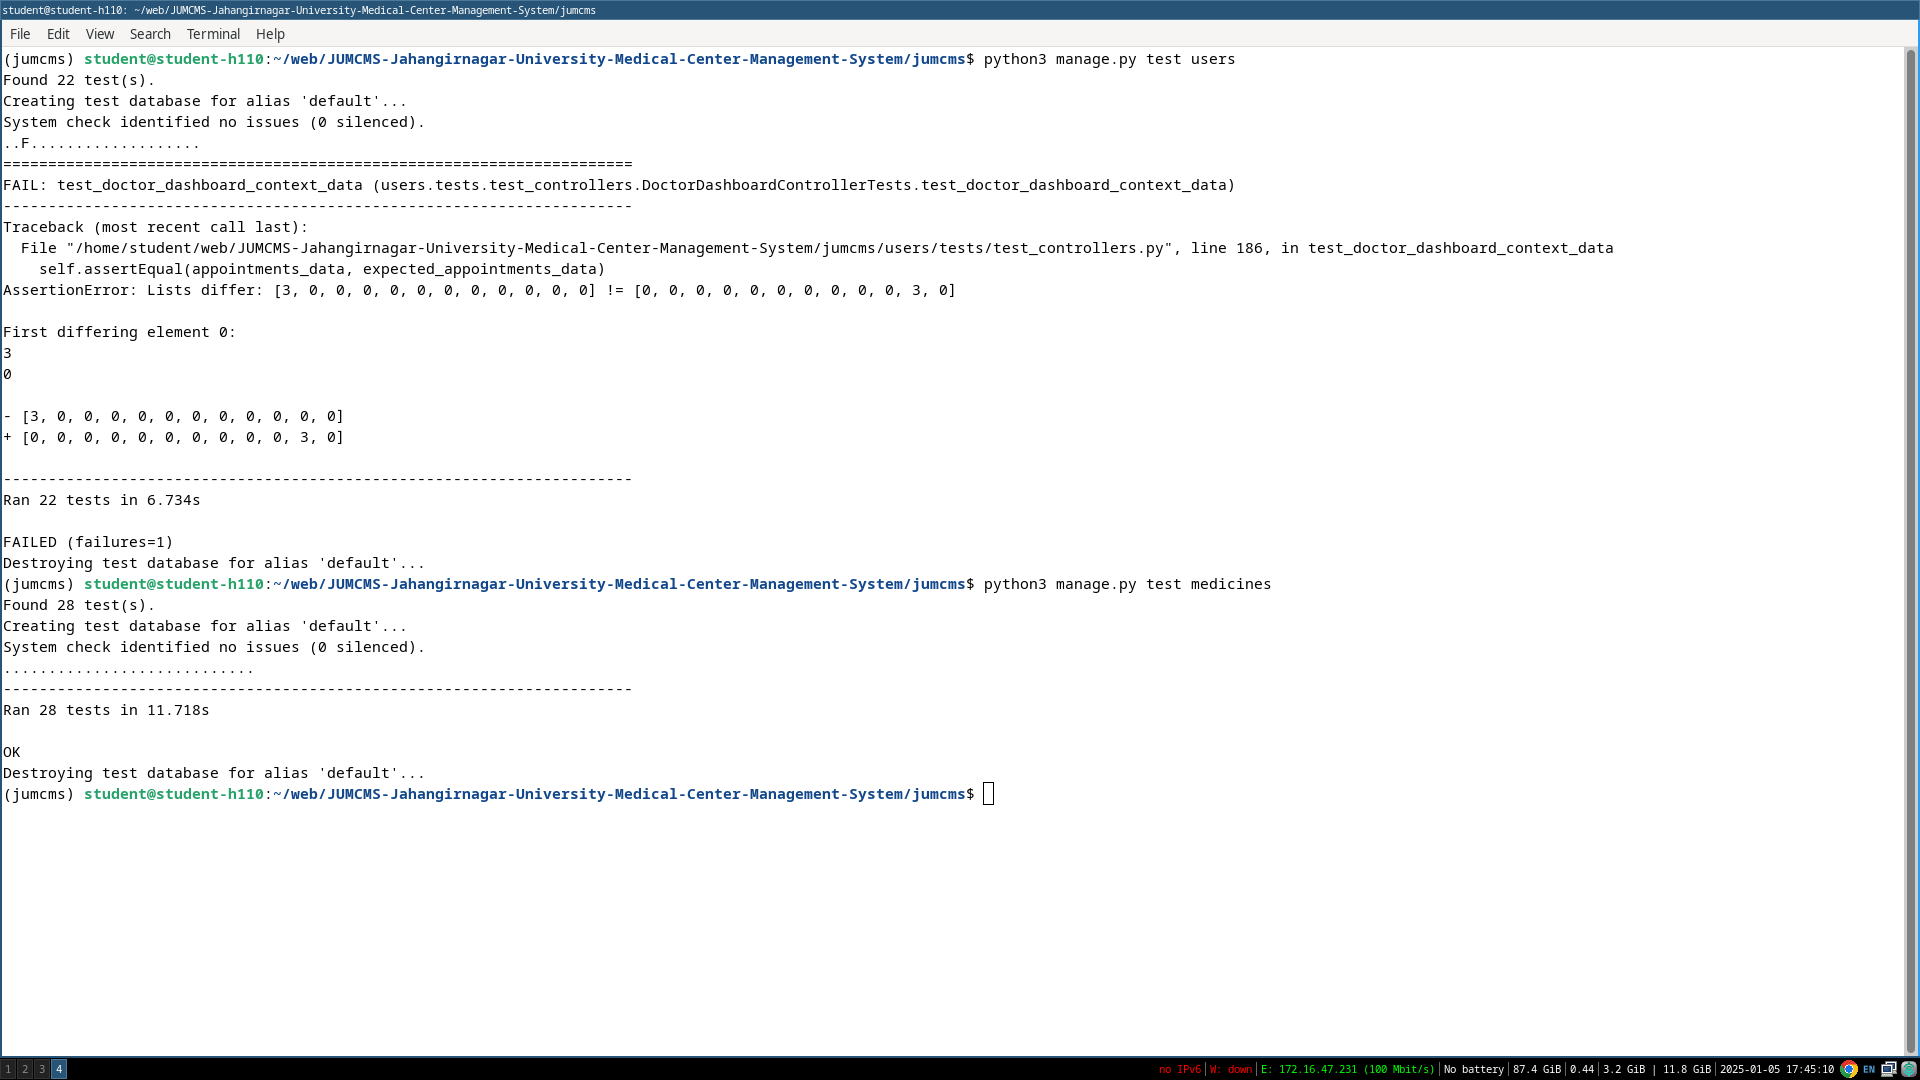
\includegraphics[width=1\textwidth]{images/TDD3.png}
    \caption{Test result for features I have implemented}
    \label{fig:tdd3}
\end{figure}

\begin{figure}[H]
    \centering
    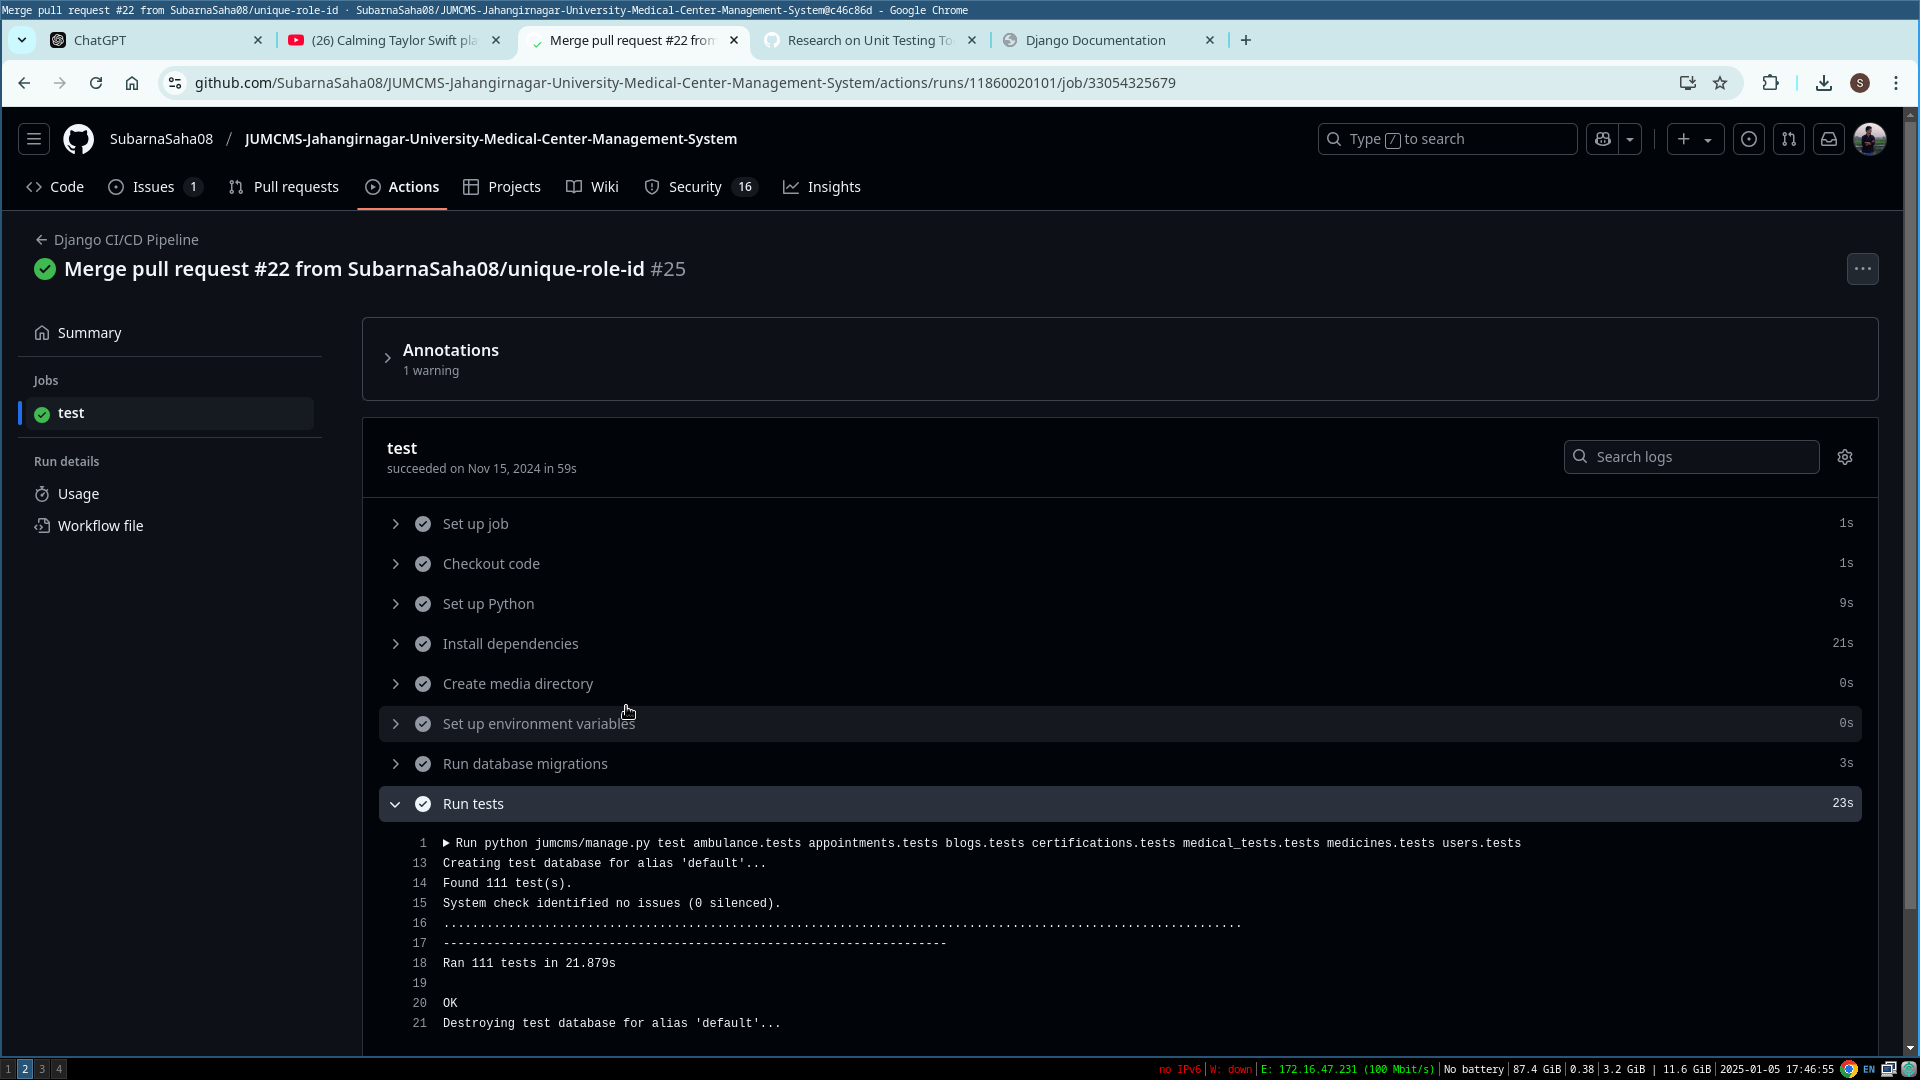
\includegraphics[width=1\textwidth]{images/TDD4.png}
    \caption{Github actions automated testing}
    \label{fig:tdd4}
\end{figure}
\section{Reflection on TDD Experience}
\begin{enumerate}
    \item \textbf{Benefits Observed}
        \begin{itemize}
            \item Improved Code Quality: Writing tests beforehand forced us to think through edge cases and
                design flaws early.
            \item Reduced Debugging Time: Automated testing identified issues at their source, reducing
                downstream debugging.
            \item Enhanced Collaboration: A shared understanding of test cases improved team alignment and
                reduced miscommunication.
            \item Incremental Progress: The “write test - write code - refactor” cycle encouraged iterative
                development and early feedback.
    \end{itemize}
    \item \textbf{Challenges Faced}
        \begin{itemize}
            \item Initial Learning Curve: Adapting to TDD required unlearning old habits and mastering new
                tools.
            \item Time Consumption: Writing tests before coding felt slower initially, especially for complex
                features.
            \item Tool Integration: Setting up a seamless CI/CD pipeline took significant effort.
    \end{itemize}
    \item \textbf{Resolution of Challenges}
        \begin{itemize}
            \item Conducted team workshops to share best practices for writing tests.
            \item Simplified test scenarios initially to reduce the learning curve.
            \item Iteratively optimized the CI/CD pipeline for faster execution.
    \end{itemize}
\end{enumerate}

 \section{TDD’s Impact on Project Outcomes}
 \begin{enumerate}
     \item \textbf{Exploring Design Solutions}
         \begin{itemize}
             \item TDD encouraged experimentation with different designs by exposing potential flaws early.
                 For example, testing revealed inefficiencies in our initial database query logic, leading to
                 significant optimizations.
         \end{itemize}
     \item \textbf{Building Confidence in Code}
         \begin{itemize}
             \item Automated tests ensured that changes or new features did not break existing functionality. This allowed the
                 team to proceed with development confidently.
         \end{itemize}
     \item \textbf{Better Collaboration}
         \begin{itemize}
             \item Comprehensive test cases served as a form of documentation, aiding communication between
                 developers and stakeholders.
         \end{itemize}
     \item \textbf{Complementary Practices}
         \begin{itemize}
             \item Continuous Integration: TDD and CI worked hand-in-hand to automate testing and integration.
             \item Code Reviews: Unit tests highlighted potential issues, making reviews more productive.
\end{itemize}
\end{enumerate}
\section{Guidelines for Good TDD Practices}
\begin{enumerate}
    \item \textbf{Write Simple and Clear Tests}
        \begin{itemize}
            \item Tests should be easy to understand, focusing on one functionality at a time.
\end{itemize}
\item \textbf{Use Mocking Wisely}
    \begin{itemize}
        \item Simulate dependencies only when necessary to avoid overcomplicating test cases.
\end{itemize}
\item \textbf{Refactor Tests Along with Code}
    \begin{itemize}
        \item Keep test cases updated to reflect changes in the application logic.
    \end{itemize}
\item \textbf{Automate Testing}
    \begin{itemize}
        \item Integrate tests into the CI/CD pipeline to ensure they are executed consistently.
\end{itemize}
\item \textbf{Involve the Team}
    \begin{itemize}
        \item Encourage collaborative test design to align on expected outcomes and edge cases.
\end{itemize}
\end{enumerate}
\section{Conclusion}
Practicing TDD during this project significantly enhanced our development process and the final product’s
quality. While it demanded an initial investment of time and effort, the long-term benefits far outweighed the
challenges. By combining TDD with CI and other agile practices, our team successfully delivered a robust and
maintainable software solution.
\end{document}
